\section{Evaluation}
To evaluate the impact flat combining has on the global data structures, we ran a series of experiments to test the raw performance of the data structures themselves under different workloads, and further measured their impact on performance of two simple graph benchmarks.

\subsection{Data Structure Throughput}
First we measured the performance of the global data structures on extremely simple workloads to understand their raw performance.

\begin{figure*}[t]
  \centering
  \begin{subfigure}[b]{0.45\textwidth}
  \centering
  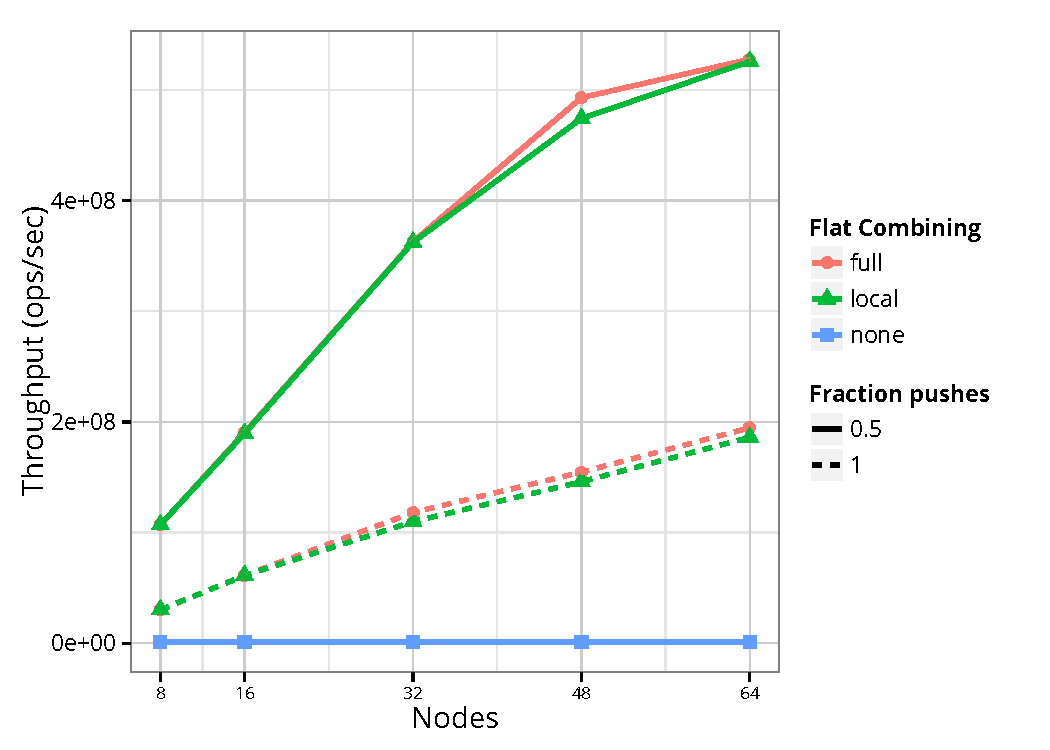
\includegraphics[width=\textwidth]{data/plots/stack_perf.pdf}
  \caption{\emph{GlobalStack.} Even with Grappa's aggregation, the stack without combining completely fails to scale. With combining, both workloads scale out to 64 nodes. The workload with roughly even pushes and pops performs best because it can do matching locally.}
  \label{fig:stack}
  \end{subfigure}%
  \hspace{0.05\textwidth}
  % ~ %add desired spacing between images, e. g. ~, \quad, \qquad etc.
  %(or a blank line to force the subfigure onto a new line)
  \begin{subfigure}[b]{0.45\textwidth}
  \centering
  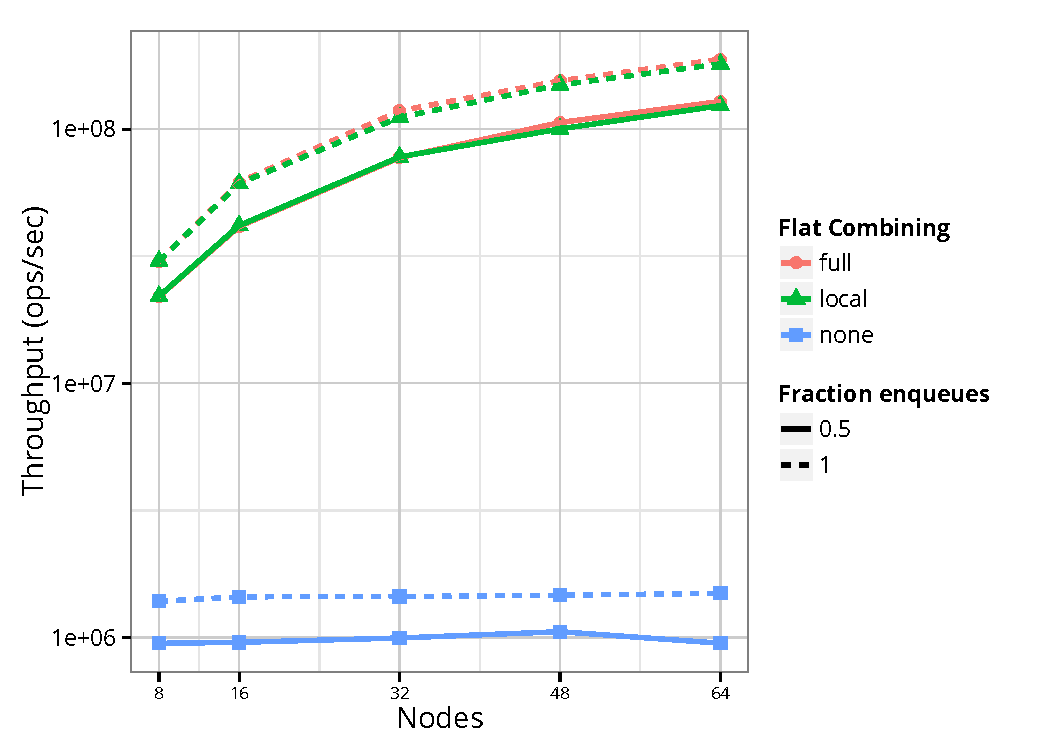
\includegraphics[width=\textwidth]{data/plots/queue_perf.pdf}
  \caption{\emph{GlobalQueue.} Same parameters as stack performance results. The queue is unable to do matching locally, but benefits from reducing the amount of synchronization that must globally serialize. The mixed workload performs worse because the current implementation serializes combined enqueue and dequeue operations.}
  \label{fig:queue}
  \end{subfigure}
  
  \begin{subfigure}[b]{0.45\textwidth}
  \centering
  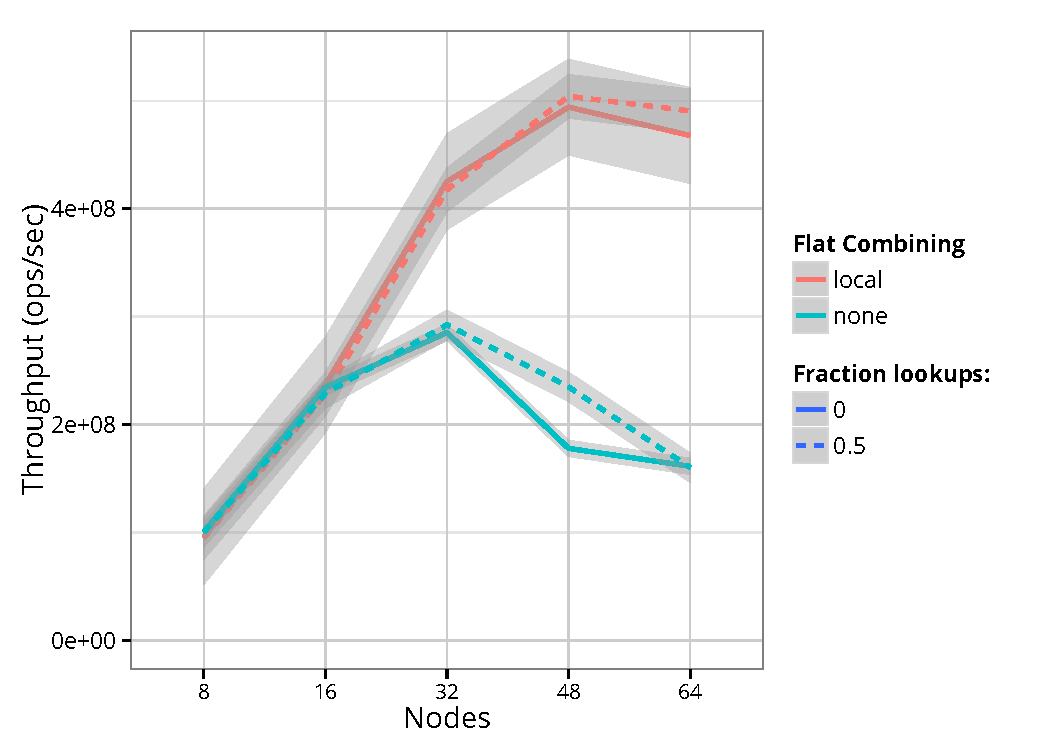
\includegraphics[width=\textwidth]{data/plots/hashset_perf.pdf}
  \caption{\emph{GlobalHashSet.} Throughput workload inserting and looking up random keys in the range 0-1024 into a global hash set with 1024 cells.
   Performance without combining scales better than the global queue or stack because synchronization happens at each hash cell, but drops off as number of destinations increases. Combining version is able to match inserts and lookups of the same key.}
    \TODO{if time: add 'delete' operation, too (show that it doesn't affect correctness or performance)}
  \label{fig:hashset}
  \end{subfigure}
  %
  \hspace{0.05\textwidth}
  %
  \begin{subfigure}[b]{0.45\textwidth}
  \centering
  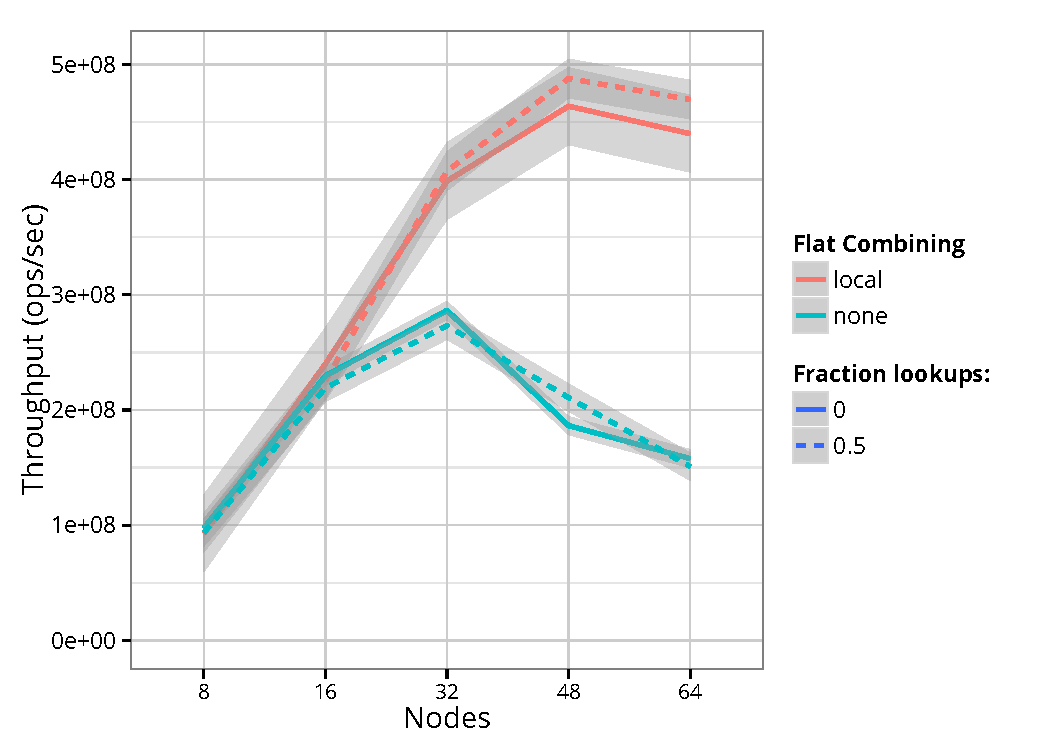
\includegraphics[width=\textwidth]{data/plots/hashmap_perf.pdf}
  \caption{\emph{GlobalHashMap.} Same workload as for the Set, but random integers as the values in the map. Performance matches that of the Set.} \TODO{try increasing size of value "payload", currently is just a tiny int64.}
  \label{fig:hashmap}
  \end{subfigure}%
  %
  \caption{
    \emph{Raw performance of global data structures on simple throughput workloads.}
    Results shown for workloads with all writes and a mix of writing and reading operations. All results are for 2048 workers per core and 16 cores per node.
    \TODO{either all with error bars or none?}
    \TODO{combine stack/queue \& set/map plots, no point in saying the same things twice.}
  }\label{fig:datastructs}
\end{figure*}

\paragraph{Queue and Stack}
The GlobalQueue and GlobalStack have very similar implementations in terms of how they are synchronized. Both benefit greatly from flat combining. This is because only one round-trip message \TODO{...}

% However, the stack is able to match up pushes and pops locally. This leads to performance on an even mix of pushes and pops far outstripping the case where all pushes are performed due to requiring vastly less communication.

\paragraph{HashSet and HashMap}
The GlobalHashSet and GlobalHashMap have the same synchronization strategy (serialization happens at each hashed location).
\TODO{...}

\subsection{Application Kernel Performance}
The impetus for this work was that naive implementations of standard data structures are insufficient for use in high-performance kernels.

\paragraph{Breadth-First Search}
\begin{figure}[t]
  \centering
  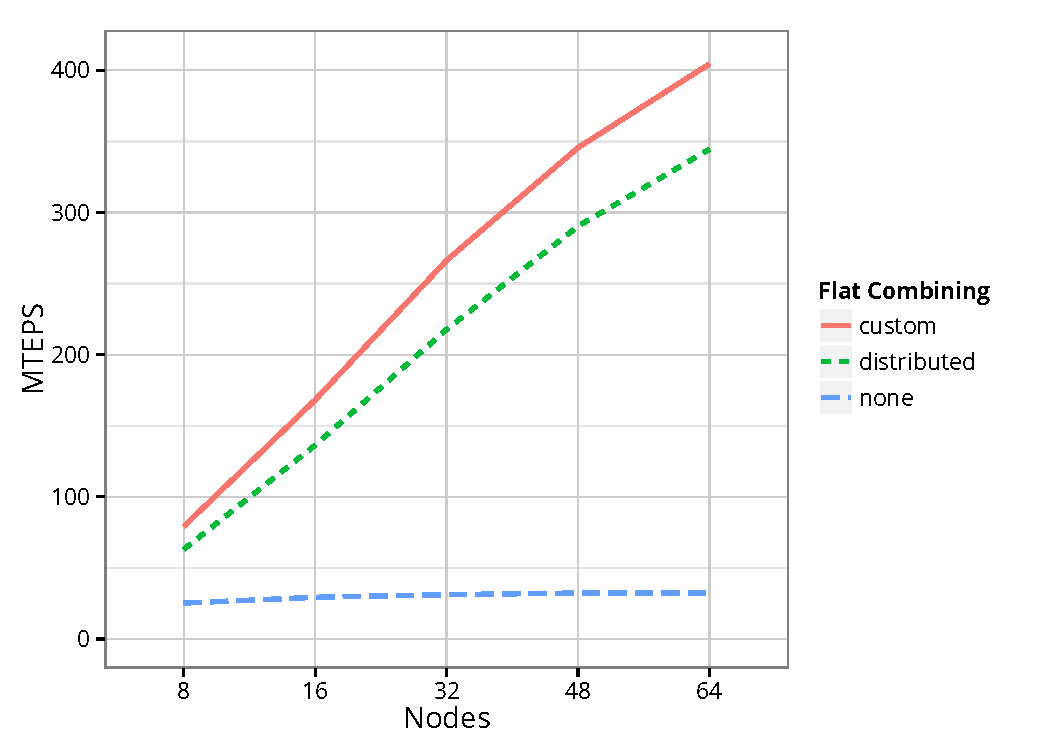
\includegraphics[width=0.5\textwidth]{data/plots/bfs_perf.pdf}
  \caption{\emph{BFS} on a Graph500-spec graph of scale 26 (64 million vertices, 1 billion edges), with the direction-optimizing BFS algorithm. Performance is measured in millions of Traversed Edges Per Second (MTEPS).}
  \label{fig:bfs_perf}
\end{figure}


\paragraph{Connected Components}

\begin{figure}[t]
  \centering
  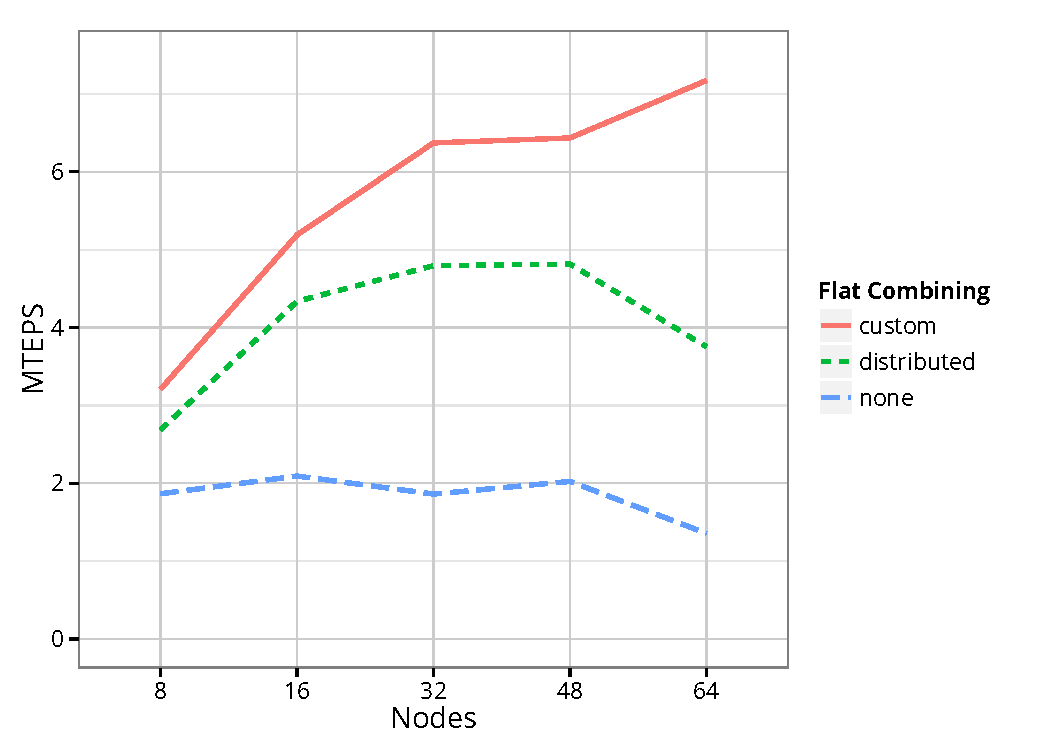
\includegraphics[width=0.5\textwidth]{data/plots/cc_perf.pdf}
  \caption{\emph{Connected Components} on the same scale 26 Graph500 graph. Performance is measured in MTEPS (parameterized by the total number of edges in the graph, independent of the algorithm used).}
  \label{fig:cc_perf}
\end{figure}

